\documentclass[10pt,]{krantz}
\usepackage{lmodern}
\usepackage{amssymb,amsmath}
\usepackage{ifxetex,ifluatex}
\usepackage{fixltx2e} % provides \textsubscript
\ifnum 0\ifxetex 1\fi\ifluatex 1\fi=0 % if pdftex
  \usepackage[T1]{fontenc}
  \usepackage[utf8]{inputenc}
\else % if luatex or xelatex
  \ifxetex
    \usepackage{mathspec}
  \else
    \usepackage{fontspec}
  \fi
  \defaultfontfeatures{Ligatures=TeX,Scale=MatchLowercase}
\fi
% use upquote if available, for straight quotes in verbatim environments
\IfFileExists{upquote.sty}{\usepackage{upquote}}{}
% use microtype if available
\IfFileExists{microtype.sty}{%
\usepackage[]{microtype}
\UseMicrotypeSet[protrusion]{basicmath} % disable protrusion for tt fonts
}{}
\PassOptionsToPackage{hyphens}{url} % url is loaded by hyperref
\usepackage[unicode=true]{hyperref}
\PassOptionsToPackage{usenames,dvipsnames}{color} % color is loaded by hyperref
\hypersetup{
            pdftitle={Análisis de Regresión con R},
            colorlinks=true,
            linkcolor=Maroon,
            citecolor=Blue,
            urlcolor=Blue,
            breaklinks=true}
\urlstyle{same}  % don't use monospace font for urls
\usepackage{natbib}
\bibliographystyle{apalike}
\usepackage{color}
\usepackage{fancyvrb}
\newcommand{\VerbBar}{|}
\newcommand{\VERB}{\Verb[commandchars=\\\{\}]}
\DefineVerbatimEnvironment{Highlighting}{Verbatim}{commandchars=\\\{\}}
% Add ',fontsize=\small' for more characters per line
\usepackage{framed}
\definecolor{shadecolor}{RGB}{248,248,248}
\newenvironment{Shaded}{\begin{snugshade}}{\end{snugshade}}
\newcommand{\KeywordTok}[1]{\textcolor[rgb]{0.13,0.29,0.53}{\textbf{#1}}}
\newcommand{\DataTypeTok}[1]{\textcolor[rgb]{0.13,0.29,0.53}{#1}}
\newcommand{\DecValTok}[1]{\textcolor[rgb]{0.00,0.00,0.81}{#1}}
\newcommand{\BaseNTok}[1]{\textcolor[rgb]{0.00,0.00,0.81}{#1}}
\newcommand{\FloatTok}[1]{\textcolor[rgb]{0.00,0.00,0.81}{#1}}
\newcommand{\ConstantTok}[1]{\textcolor[rgb]{0.00,0.00,0.00}{#1}}
\newcommand{\CharTok}[1]{\textcolor[rgb]{0.31,0.60,0.02}{#1}}
\newcommand{\SpecialCharTok}[1]{\textcolor[rgb]{0.00,0.00,0.00}{#1}}
\newcommand{\StringTok}[1]{\textcolor[rgb]{0.31,0.60,0.02}{#1}}
\newcommand{\VerbatimStringTok}[1]{\textcolor[rgb]{0.31,0.60,0.02}{#1}}
\newcommand{\SpecialStringTok}[1]{\textcolor[rgb]{0.31,0.60,0.02}{#1}}
\newcommand{\ImportTok}[1]{#1}
\newcommand{\CommentTok}[1]{\textcolor[rgb]{0.56,0.35,0.01}{\textit{#1}}}
\newcommand{\DocumentationTok}[1]{\textcolor[rgb]{0.56,0.35,0.01}{\textbf{\textit{#1}}}}
\newcommand{\AnnotationTok}[1]{\textcolor[rgb]{0.56,0.35,0.01}{\textbf{\textit{#1}}}}
\newcommand{\CommentVarTok}[1]{\textcolor[rgb]{0.56,0.35,0.01}{\textbf{\textit{#1}}}}
\newcommand{\OtherTok}[1]{\textcolor[rgb]{0.56,0.35,0.01}{#1}}
\newcommand{\FunctionTok}[1]{\textcolor[rgb]{0.00,0.00,0.00}{#1}}
\newcommand{\VariableTok}[1]{\textcolor[rgb]{0.00,0.00,0.00}{#1}}
\newcommand{\ControlFlowTok}[1]{\textcolor[rgb]{0.13,0.29,0.53}{\textbf{#1}}}
\newcommand{\OperatorTok}[1]{\textcolor[rgb]{0.81,0.36,0.00}{\textbf{#1}}}
\newcommand{\BuiltInTok}[1]{#1}
\newcommand{\ExtensionTok}[1]{#1}
\newcommand{\PreprocessorTok}[1]{\textcolor[rgb]{0.56,0.35,0.01}{\textit{#1}}}
\newcommand{\AttributeTok}[1]{\textcolor[rgb]{0.77,0.63,0.00}{#1}}
\newcommand{\RegionMarkerTok}[1]{#1}
\newcommand{\InformationTok}[1]{\textcolor[rgb]{0.56,0.35,0.01}{\textbf{\textit{#1}}}}
\newcommand{\WarningTok}[1]{\textcolor[rgb]{0.56,0.35,0.01}{\textbf{\textit{#1}}}}
\newcommand{\AlertTok}[1]{\textcolor[rgb]{0.94,0.16,0.16}{#1}}
\newcommand{\ErrorTok}[1]{\textcolor[rgb]{0.64,0.00,0.00}{\textbf{#1}}}
\newcommand{\NormalTok}[1]{#1}
\usepackage{longtable,booktabs}
% Fix footnotes in tables (requires footnote package)
\IfFileExists{footnote.sty}{\usepackage{footnote}\makesavenoteenv{long table}}{}
\usepackage{graphicx,grffile}
\makeatletter
\def\maxwidth{\ifdim\Gin@nat@width>\linewidth\linewidth\else\Gin@nat@width\fi}
\def\maxheight{\ifdim\Gin@nat@height>\textheight\textheight\else\Gin@nat@height\fi}
\makeatother
% Scale images if necessary, so that they will not overflow the page
% margins by default, and it is still possible to overwrite the defaults
% using explicit options in \includegraphics[width, height, ...]{}
\setkeys{Gin}{width=\maxwidth,height=\maxheight,keepaspectratio}
\IfFileExists{parskip.sty}{%
\usepackage{parskip}
}{% else
\setlength{\parindent}{0pt}
\setlength{\parskip}{6pt plus 2pt minus 1pt}
}
\setlength{\emergencystretch}{3em}  % prevent overfull lines
\providecommand{\tightlist}{%
  \setlength{\itemsep}{0pt}\setlength{\parskip}{0pt}}
\setcounter{secnumdepth}{5}
% Redefines (sub)paragraphs to behave more like sections
\ifx\paragraph\undefined\else
\let\oldparagraph\paragraph
\renewcommand{\paragraph}[1]{\oldparagraph{#1}\mbox{}}
\fi
\ifx\subparagraph\undefined\else
\let\oldsubparagraph\subparagraph
\renewcommand{\subparagraph}[1]{\oldsubparagraph{#1}\mbox{}}
\fi

% set default figure placement to htbp
\makeatletter
\def\fps@figure{htbp}
\makeatother

\usepackage{booktabs}
\usepackage[spanish]{babel}
\decimalpoint
\selectlanguage{spanish}

% Comandos para escribir nombres de paquetes, programas y codigos
\newcommand{\pkg}[1]{{\normalfont\fontseries{b}\selectfont #1}}
\let\proglang=\textsf
\let\code=\texttt


\usepackage{booktabs}
\usepackage{longtable}
\usepackage[bf,singlelinecheck=off]{caption}

\usepackage{framed,color}
\definecolor{shadecolor}{RGB}{248,248,248}

\renewcommand{\textfraction}{0.05}
\renewcommand{\topfraction}{0.8}
\renewcommand{\bottomfraction}{0.8}
\renewcommand{\floatpagefraction}{0.75}

\renewenvironment{quote}{\begin{VF}}{\end{VF}}
\let\oldhref\href
\renewcommand{\href}[2]{#2\footnote{\url{#1}}}

\ifxetex
  \usepackage{letltxmacro}
  \setlength{\XeTeXLinkMargin}{1pt}
  \LetLtxMacro\SavedIncludeGraphics\includegraphics
  \def\includegraphics#1#{% #1 catches optional stuff (star/opt. arg.)
    \IncludeGraphicsAux{#1}%
  }%
  \newcommand*{\IncludeGraphicsAux}[2]{%
    \XeTeXLinkBox{%
      \SavedIncludeGraphics#1{#2}%
    }%
  }%
\fi

\makeatletter
\newenvironment{kframe}{%
\medskip{}
\setlength{\fboxsep}{.8em}
 \def\at@end@of@kframe{}%
 \ifinner\ifhmode%
  \def\at@end@of@kframe{\end{minipage}}%
  \begin{minipage}{\columnwidth}%
 \fi\fi%
 \def\FrameCommand##1{\hskip\@totalleftmargin \hskip-\fboxsep
 \colorbox{shadecolor}{##1}\hskip-\fboxsep
     % There is no \\@totalrightmargin, so:
     \hskip-\linewidth \hskip-\@totalleftmargin \hskip\columnwidth}%
 \MakeFramed {\advance\hsize-\width
   \@totalleftmargin\z@ \linewidth\hsize
   \@setminipage}}%
 {\par\unskip\endMakeFramed%
 \at@end@of@kframe}
\makeatother

\renewenvironment{Shaded}{\begin{kframe}}{\end{kframe}}

%%%%%

\newenvironment{rmdblock}[1]
  {
  \begin{itemize}
  \renewcommand{\labelitemi}{
    \raisebox{-.7\height}[0pt][0pt]{
      {\setkeys{Gin}{width=3em,keepaspectratio}\includegraphics{images/#1}}
    }
  }
  \setlength{\fboxsep}{1em}
  \begin{kframe}
  \item
  }
  {
  \end{kframe}
  \end{itemize}
  }
\newenvironment{rmdnote}
  {\begin{rmdblock}{note}}
  {\end{rmdblock}}
\newenvironment{rmdcaution}
  {\begin{rmdblock}{caution}}
  {\end{rmdblock}}
\newenvironment{rmdimportant}
  {\begin{rmdblock}{important}}
  {\end{rmdblock}}
\newenvironment{rmdtip}
  {\begin{rmdblock}{tip}}
  {\end{rmdblock}}
\newenvironment{rmdwarning}
  {\begin{rmdblock}{warning}}
  {\end{rmdblock}}


%%%%%

\usepackage{makeidx}
\makeindex

\urlstyle{tt}

\usepackage{amsthm}
\makeatletter
\def\thm@space@setup{%
  \thm@preskip=8pt plus 2pt minus 4pt
  \thm@postskip=\thm@preskip
}
\makeatother

\frontmatter

\title{Análisis de Regresión con R}
\author{Mauricio Mazo Lopera\\
Freddy Hernández Barajas}
\date{2018-10-01}

\let\BeginKnitrBlock\begin \let\EndKnitrBlock\end
\begin{document}
\maketitle

% you may need to leave a few empty pages before the dedication page

%\cleardoublepage\newpage\thispagestyle{empty}\null
%\cleardoublepage\newpage\thispagestyle{empty}\null
%\cleardoublepage\newpage
\thispagestyle{empty}

\begin{center}

aquí la dedicatoria o pensamiento de mauro.

Mauricio Mazo Lopera

\vspace{1cm}


Gracias a Dios por todo lo que me ha dado!

Freddy Hernández Barajas

%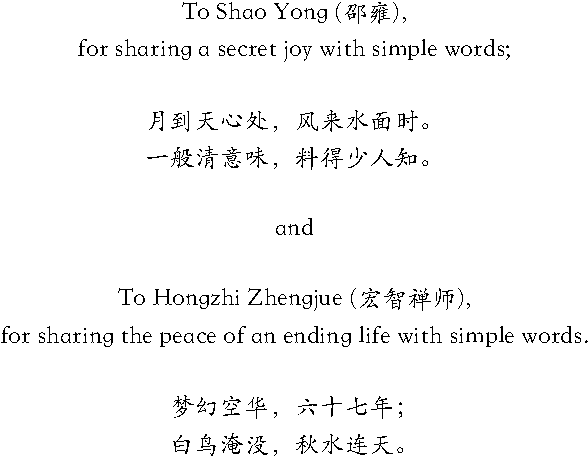
\includegraphics{images/dedication.pdf}
\end{center}

\setlength{\abovedisplayskip}{-5pt}
\setlength{\abovedisplayshortskip}{-5pt}

{
\hypersetup{linkcolor=black}
\setcounter{tocdepth}{2}
\tableofcontents
}
\listoftables
\listoffigures
\chapter*{Prefacio}\label{prefacio}


Este libro está destinado para estudiantes de ingeniería y estadística
que deseen aprender la teoría sobre modelos de regresión y la forma de
aplicarlos por medio de lenguage de programación \proglang{R}.

\section*{Estructura del libro}\label{estructura-del-libro}


En el capítulo \ref{rls} se presenta el modelo de regresión lineal
simple y en el Capítulo \ref{rlm} se generaliza el modelo básico a
múltiples variables. El Capítulo \ref{resid} muestra cómo se calculan
los residuales en un modelo y la forma en que éstos permiten saber si el
modelo está bien definido. En el capítulo \ref{demos} se encuentran
todas las demostraciones menciondas en el libro.

\section*{Software information and
conventions}\label{software-information-and-conventions}


Para realizar este libro usamos los paquetes \textbf{knitr}\index{knitr}
\citep{xie2015} y \textbf{bookdown}\index{bookdown} \citep{R-bookdown}
que permiten unir la ventajas de \LaTeX y \proglang{R} en un mismo
archivo.

En todo el libro se presentarán códigos que el lector puede copiar y
pegar en su consola de \proglang{R} para obtener los mismos resultados
aquí presentados. Los códigos se destacan en una caja de color beis (o
beige) similar a la mostrada a continuación.

\begin{Shaded}
\begin{Highlighting}[]
\DecValTok{4} \OperatorTok{+}\StringTok{ }\DecValTok{6}
\NormalTok{a <-}\StringTok{ }\KeywordTok{c}\NormalTok{(}\DecValTok{1}\NormalTok{, }\DecValTok{5}\NormalTok{, }\DecValTok{6}\NormalTok{)}
\DecValTok{5} \OperatorTok{*}\StringTok{ }\NormalTok{a}
\DecValTok{1}\OperatorTok{:}\DecValTok{10}
\end{Highlighting}
\end{Shaded}

Los resultados o salidas obtenidos de cualquier código se destacan con
dos símbolos de númeral (\texttt{\#\#}) al inicio de cada línea o
renglón, esto quiere decir que todo lo que inicie con \texttt{\#\#} son
resultados obtenidos y \textbf{NO} los debe copiar. Abajo se muestran
los resultados obtenidos luego de correr el código anterior.

\begin{verbatim}
## [1] 10
\end{verbatim}

\begin{verbatim}
## [1]  5 25 30
\end{verbatim}

\begin{verbatim}
##  [1]  1  2  3  4  5  6  7  8  9 10
\end{verbatim}

\section*{Bloques informativos}\label{bloques-informativos}


En varias partes del libro usaremos bloques informativos para resaltar
algún aspecto importante. Abajo se encuentra un ejemplo de los bloques y
su significado.

\BeginKnitrBlock{rmdnote}
Este bloque sirve para una nota aclaratoria.
\EndKnitrBlock{rmdnote}

\BeginKnitrBlock{rmdtip}
Este bloque sirve para una sugerencia.
\EndKnitrBlock{rmdtip}

\BeginKnitrBlock{rmdwarning}
Este bloque sirve para una advertencia.
\EndKnitrBlock{rmdwarning}

\section*{Agradecimientos}\label{agradecimientos}


Agradecemos a nuestros estudiantes, profesores y colegas que han leído
el manuscrito y se han tomado el trabajo de escribirnos dándonos sus
sugerencias y comentarios para mejorar continuamente este material.

\BeginKnitrBlock{flushright}
Mauricio Mazo Lopera

Freddy Hernández Barajas
\EndKnitrBlock{flushright}

\chapter*{Sobre los autores}\label{sobre-los-autores}


Mauricio Mazo Lopera es profesor xxxx de la Universidad Nacional de
Colombia sede Medellín, adscrito a la Escuela de Estadística de la
Facultad de Ciencias.

mail:
\href{mailto:sucorreo@unal.edu.co}{\nolinkurl{sucorreo@unal.edu.co}}

\vspace{1cm}

Freddy Hernández Barajas es profesor asistente de la Universidad
Nacional de Colombia sede Medellín, adscrito a la Escuela de Estadística
de la Facultad de Ciencias.

mail:
\href{mailto:fhernanb@unal.edu.co}{\nolinkurl{fhernanb@unal.edu.co}}

webpage: \url{https://fhernanb.github.io/}

\mainmatter

\chapter{Introducción}\label{intro}

Aquí va la introducción del libro. Ensayo 1

\BeginKnitrBlock{rmdwarning}
Mauro, yo le recomiendo que haga cambios pequeños y luego build el libro
para que pueda ver el efecto y así detectar los errores más fácil.
\EndKnitrBlock{rmdwarning}

\chapter{Regresión lineal simple}\label{rls}

Considere una muestra de tamaño \(n\), el modelo de regresión lineal
simple para el \(i\)-ésimo individuo está dado por:

\[y_i=\beta_0+\beta_1 x_i + e_i,\ \ \text{para $i=1, \ldots, n$}\]

donde los supuestos del modelo son:

\begin{itemize}
\item
  \(e_i\) tiene una distribución normal para cada \(i=1, \ldots, n\)
\item
  \(E(e_i)=0\) y \(Var(e_i)=\sigma^2\), de donde
  \(E(Y_i)=\beta_0+\beta_1X_i\) y \(Var(Y_i)=\sigma^2\)
\item
  Los \(e_1, e_2, \ldots, e_n\) son independientes.
\end{itemize}

Podemos agregar figuras directamente así:

\begin{Shaded}
\begin{Highlighting}[]
\NormalTok{y <-}\StringTok{ }\KeywordTok{rnorm}\NormalTok{(}\DecValTok{100}\NormalTok{)}
\KeywordTok{plot}\NormalTok{(}\KeywordTok{density}\NormalTok{(y), }\DataTypeTok{lwd=}\DecValTok{2}\NormalTok{, }\DataTypeTok{col=}\StringTok{'blue3'}\NormalTok{)}
\end{Highlighting}
\end{Shaded}

\begin{figure}
\centering
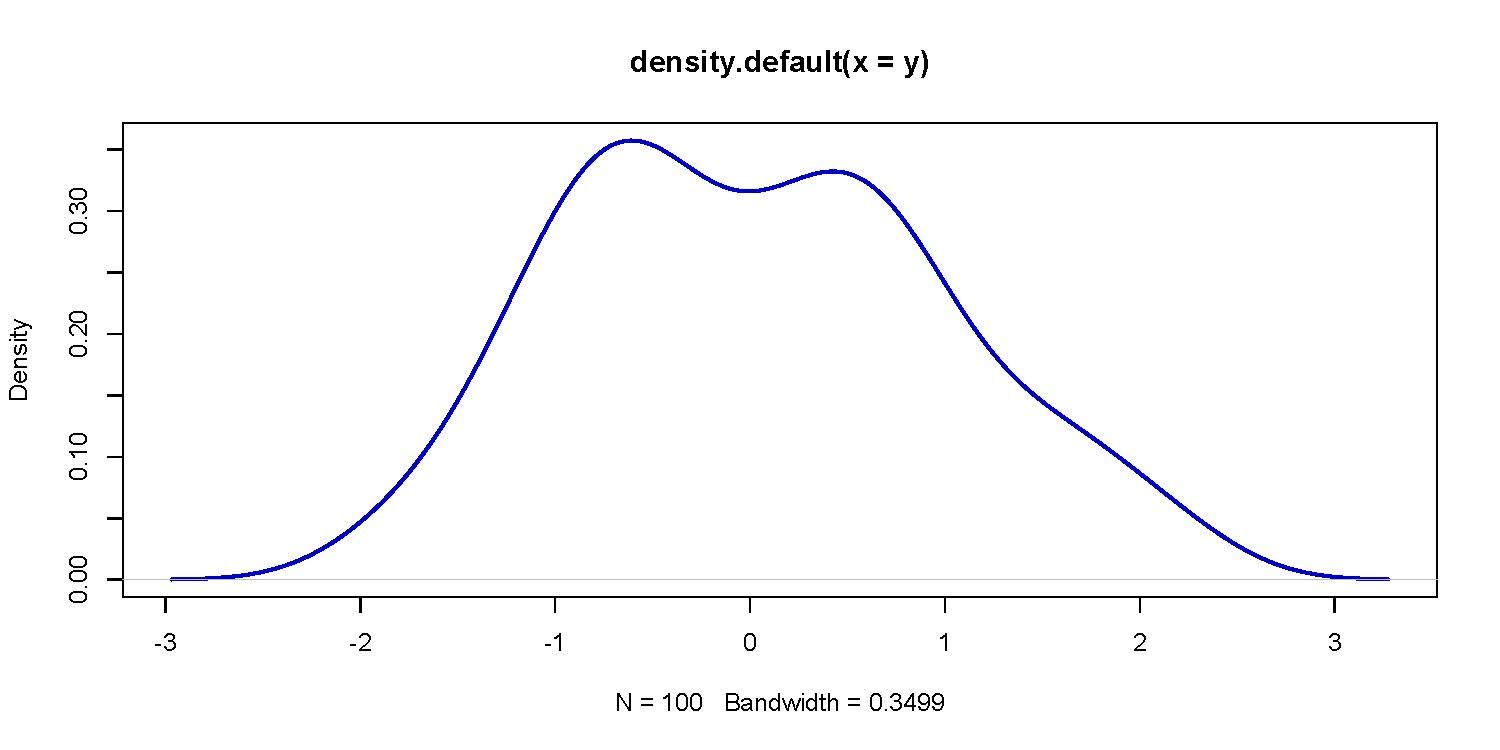
\includegraphics{analisis_de_regresion_con_R_files/figure-latex/prueba1-1.pdf}
\caption{\label{fig:prueba1}Hola Mauricio, esto es una prueba.}
\end{figure}

\section*{Ejemplo}\label{ejemplo}


Aquí va el texto del ejemplo.

\section*{Ejemplo}\label{ejemplo-1}


Aquí va el texto del ejemplo.

\BeginKnitrBlock{rmdnote}
Mauro, los ejemplos no se numeran mientras que las secciones si. Si
usted coloca \{-\} en una sección no aparecerá número.
\EndKnitrBlock{rmdnote}

\chapter{Regresión lineal múltiple}\label{rlm}

Se pueden incluir tablas con datos de la siguiente manera.

\begin{Shaded}
\begin{Highlighting}[]
\NormalTok{knitr}\OperatorTok{::}\KeywordTok{kable}\NormalTok{(}
  \KeywordTok{head}\NormalTok{(mtcars[, }\DecValTok{1}\OperatorTok{:}\DecValTok{8}\NormalTok{], }\DecValTok{10}\NormalTok{), }\DataTypeTok{booktabs =} \OtherTok{TRUE}\NormalTok{,}
  \DataTypeTok{caption =} \StringTok{'A table of the first 10 rows of the mtcars data.'}
\NormalTok{)}
\end{Highlighting}
\end{Shaded}

\begin{table}

\caption{\label{tab:unnamed-chunk-9}A table of the first 10 rows of the mtcars data.}
\centering
\begin{tabular}[t]{lrrrrrrrr}
\toprule
  & mpg & cyl & disp & hp & drat & wt & qsec & vs\\
\midrule
Mazda RX4 & 21.0 & 6 & 160.0 & 110 & 3.90 & 2.620 & 16.46 & 0\\
Mazda RX4 Wag & 21.0 & 6 & 160.0 & 110 & 3.90 & 2.875 & 17.02 & 0\\
Datsun 710 & 22.8 & 4 & 108.0 & 93 & 3.85 & 2.320 & 18.61 & 1\\
Hornet 4 Drive & 21.4 & 6 & 258.0 & 110 & 3.08 & 3.215 & 19.44 & 1\\
Hornet Sportabout & 18.7 & 8 & 360.0 & 175 & 3.15 & 3.440 & 17.02 & 0\\
\addlinespace
Valiant & 18.1 & 6 & 225.0 & 105 & 2.76 & 3.460 & 20.22 & 1\\
Duster 360 & 14.3 & 8 & 360.0 & 245 & 3.21 & 3.570 & 15.84 & 0\\
Merc 240D & 24.4 & 4 & 146.7 & 62 & 3.69 & 3.190 & 20.00 & 1\\
Merc 230 & 22.8 & 4 & 140.8 & 95 & 3.92 & 3.150 & 22.90 & 1\\
Merc 280 & 19.2 & 6 & 167.6 & 123 & 3.92 & 3.440 & 18.30 & 1\\
\bottomrule
\end{tabular}
\end{table}

\section*{Ejemplo}\label{ejemplo-2}


Aquí va el texto del ejemplo.

\section*{Ejemplo}\label{ejemplo-3}


Aquí va el texto del ejemplo.

\chapter{Comprobación de la adecuación del modelo}\label{resid}

\section{Definición de residuales}\label{definicion-de-residuales}

Aquí el contenido de la sección.

\section{Métodos para escalr
residuales}\label{metodos-para-escalr-residuales}

Aquí el contenido de la sección.

\section{Gráficas de residuales}\label{graficas-de-residuales}

Aquí el contenido de la sección.

\section{Estadística PRESS}\label{estadistica-press}

Aquí el contenido de la sección.

\chapter{Transformaciones}\label{transf}

Bla bla bla.

\chapter{Demostraciones}\label{demos}

\section{Demostración de los estimadores de máxima
verosimilitud}\label{demostracion-de-los-estimadores-de-maxima-verosimilitud}

Aquí la demostración.

Mauricio, usted puede referenciar esta demostración en cualquier
capítulo usando una instrucción sencilla.

\section{Demostración de la distribución de los ja ja
ja}\label{demostracion-de-la-distribucion-de-los-ja-ja-ja}

Aquí la demostración.

\bibliography{book.bib,packages.bib}

\backmatter
\printindex

\end{document}
